\chapter*{About the Author}
\addcontentsline{toc}{chapter}{About the Author}
\chaptermark{About the Author}

\begin{wrapfigure}{l}{0.32\textwidth}
    \centering
    \vspace{-10pt}
    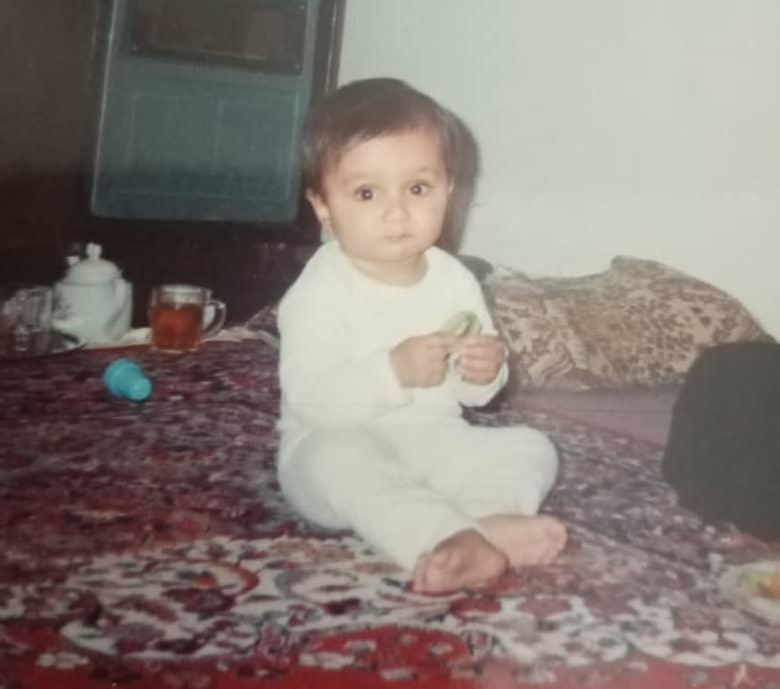
\includegraphics[width=\linewidth]{images/author-photo.jpg}
\end{wrapfigure}
{\small \linespread{0.96}\selectfont
\textbf{Mahdi} is a backend engineer, open-source developer, and lifelong
computer enthusiast from Iran, currently pursuing a Bachelor's degree in Computer
Engineering. His fascination with computers began long before university. From the age
of four, computers were a constant companion first as a source of curiosity and games,
and later as a window into understanding how technology works. Long before writing software, he enjoyed writing stories. At the age of thirteen or
fourteen, he wrote his first book, a fictional story centered around dinosaurs. Although
far removed from programming, that early experience cultivated a lasting appreciation
for exploration, creativity, and the habit of pursuing ideas simply because they were
interesting. At nineteen, upon entering university, a childhood fascination with computers evolved
into a serious interest in software engineering. Alongside his academic studies, he began
a largely self-directed journey into programming, driven not by formal curricula but by
curiosity. Seeking structure for his studies, he created a personal roadmap repository,
\textit{Algorithms \& Data Structures}, which gradually became both a learning journal
and a guide through the broader landscape of computer science.\\
That journey introduced him to a wide range of programming languages and paradigms.
Beyond modern languages, he explored older and less common systems such as Perl,
Haskell, Ada, and even a small amount of assembly language. Through C and C++, he
built numerous small projects and developed a growing interest in the lower layers of
computing how abstractions emerge from hardware and how software ultimately interacts
with the machine beneath.\\
Over the years, his work naturally gravitated toward developer tooling and infrastructure.
He has built command-line utilities, backend frameworks, validation systems, HTTP
clients, file-tree explorers, moderation services, and other software intended to make
development environments simpler and easier to reason about. Much of this work has been
released as open source and shared with the broader programming community.\\
Eventually, a deceptively simple question emerged:

\begin{center}
    \emph{What is an array?}
\end{center}
At first, the question appeared trivial. But pursuing it led far beyond the boundaries
of introductory programming. Following that thread revealed a path stretching from
high-level languages to memory layouts, from CPU caches and transistor physics to GPUs,
SIMD instructions, tensor cores, and even the foundations of quantum computation.\\
\textit{Arliz} is the written record of that journey an attempt to follow one simple
question as far as possible, and to understand not merely how arrays are used, but what
they truly are.
}

\clearpage